\documentclass[11pt]{beamer}

\usetheme{Luebeck}

\usepackage[utf8]{inputenc}
\usepackage[english]{babel}
\usepackage{amsmath}
\usepackage{amsfonts}
\usepackage{amssymb}
\usepackage{caption}

\usepackage{sansmathaccent}
\pdfmapfile{+sansmathaccent.map}

\usepackage{subfig}
\captionsetup{labelformat=empty}
\usepackage{xcolor}

\usepackage[style=alphabetic,backend=biber]{biblatex}
\addbibresource{slides.bib}

%% Defining new colors %%
\definecolor{Orange}{RGB}{255,140,30}
\definecolor{DarkBlue}{RGB}{35,10,73}
\definecolor{LightBlue}{RGB}{204,204,255}
\definecolor{DarkRed}{RGB}{135,13,13}
\definecolor{LightGray}{RGB}{210,210,224}

\setbeamercolor{normal text}{fg=black,bg=LightGray}
\setbeamercolor{structure}{fg=DarkBlue}
\setbeamercolor{palette quaternary}{fg=white, bg=DarkBlue}
\setbeamercolor{title}{bg=DarkBlue,fg=white}
\setbeamercolor{title page}{fg=LightBlue}
\setbeamercolor{alerted text}{fg=DarkRed}

\newcommand{\citem}{\textcolor{DarkBlue}{\(\blacktriangleright\)}}
\newcommand{\calertitem}{\textcolor{DarkRed}{\(\blacktriangleright\)}}


%% REVISION MACROS

\newcommand{\todo}[1]{\textcolor{red}{\textbf{ToDo}\ifx&#1&\else~[\emph{#1} ]~\fi}}
\newcommand{\fixme}[1]{\textcolor{purple}{\textbf{FixMe}\ifx&#1&\else~[ \emph{#1} ]~\fi}}


%% Tikz for picture drawing %%
\usepackage{tikz}
\usetikzlibrary{arrows}

%%
\title{Data Skew in Map-Reduce}
\subtitle{Cloud and Big Data --- M1RI}
\date{April 4th, 2017}
\author{Florestan De Moor \& Jérémy Thibault}

\titlegraphic{
\includegraphics[scale=0.6]{ens} \hspace{2cm} 
\includegraphics[scale=0.15]{univ-rennes1}}

%%
\defbeamertemplate*{title page}{customized}[1][]
{
  \vfill

  \usebeamerfont{title}\LARGE\usebeamercolor[fg]{subtitle}\inserttitle\par
  \hspace*{0.05\linewidth}\usebeamerfont{subtitle}\insertsubtitle\par
  \noindent\rule[0.5ex]{0.8\linewidth}{0.5pt}

  \vfill

  \usebeamerfont{author}\small\insertauthor\par
  \usebeamerfont{institute}\small\insertinstitute\par
  \hspace*{0.05\linewidth}\usebeamerfont{date}\small\textit{\insertdate}\par

  \vfill

  \usebeamercolor[fg]{titlegraphic}\inserttitlegraphic%
}

\useoutertheme[subsection=false]{smoothbars}
\setbeamertemplate{navigation symbols}{}
\makeatletter
\setbeamertemplate{footline}
{%
  \pgfuseshading{beamer@barshade}%
  \tiny
  \ifbeamer@sb@subsection%
    \vskip-7.75ex%chktex 41
  \else%
    \vskip-7ex%chktex 41
  \fi%
  \ifbeamer@sb@subsection%
    \begin{beamercolorbox}[ignorebg,ht=2.125ex,dp=1.125ex,%
      leftskip=.3cm,rightskip=.3cm plus1fil]{subsection in head/foot}
      \usebeamerfont{subsection in head/foot}\insertsubsectionhead%
    \end{beamercolorbox}%
  \fi%
  \begin{beamercolorbox}[ignorebg,ht=2.25ex,dp=3.75ex]{section in head/foot}
    \insertnavigation{0.9\paperwidth}
    \hfill\insertframenumber\hspace*{0.3cm}%
  \end{beamercolorbox}%
}%
\setbeamertemplate{headline}{}
%\setbeamertemplate{footline}{}
\makeatother

\setbeamertemplate{caption}{\raggedright\insertcaption\par}
\setbeamertemplate{bibliography item}[text]

\newenvironment<>{cblock}[1]{%
      \par%
      \usebeamercolor[fg]{structure} \textbf{#1}\par
      \noindent\rule[0.5ex]{0.8\linewidth}{1pt}

      \usebeamercolor[fg]{normal text}}
    {\par}%

\newenvironment<>{calertblock}[1]{%
      \par%
      \usebeamercolor[fg]{alerted text} \textbf{#1}\par
      \noindent\rule[0.5ex]{0.8\linewidth}{1pt}

      \usebeamercolor[fg]{normal text}}
    {\par}%

\graphicspath{{img/}}

\begin{document}

%%%%%%%%%%%%%%%%%%%%%%%%%%%%%%%%%%%%%%%%%%%%%%%%%%%%%%%%%%%%

\setbeamercolor{background canvas}{bg=DarkBlue}
\begin{frame}[plain,noframenumbering]
    \maketitle
\end{frame}
\setbeamercolor{background canvas}{bg=LightGray}

%%%%%%%%%%%%%%%%%%%%%%%%%%%%%%%%%%%%%%%%%%%%%%%%%%%%%%%%%%%%

\section{Introduction}

%%%%%%%%%%%%%%%%%%%%

\begin{frame}{Map-Reduce~\cite{Dean:2008:MSD:1327452.1327492}}

\todo{}

\begin{figure}
    \centering
    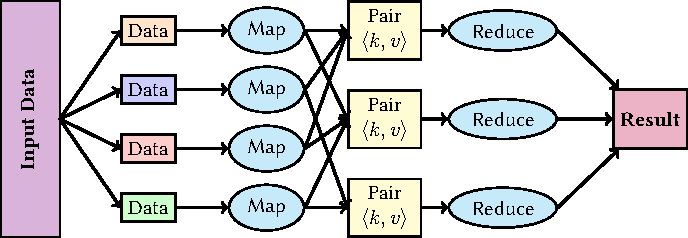
\includegraphics[width=0.8\textwidth]{map_reduce}
    \caption{Map-Reduce overview [Wikipedia]}\label{img:map_reduce}
\end{figure}

\end{frame}

\begin{frame}{Skewness Definition [Wikipedia]}

\citem{} \textbf{Asymmetry} of a probability distribution or a dataset distribution

\vfill \pause%

\begin{cblock}{Skew Example}
\begin{figure}
    \centering
    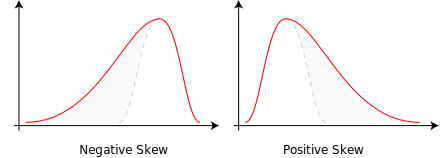
\includegraphics[width=0.7\textwidth]{skewness}
    \caption{Example of negative and positive skewness in a probability distribution}\label{img:skewness_def}
\end{figure}
\end{cblock}

\end{frame}

%%%%%%%%%%%%%%%%%%%%

\begin{frame}{Outline}
    \tableofcontents
\end{frame}

%%%%%%%%%%%%%%%%%%%%%%%%%%%%%%%%%%%%%%%%

\section{Data Skew Overview}

\begin{frame}{Outline}
    \tableofcontents[currentsection]
\end{frame}

\subsection{Challenges}

%%%%%%%%%%%%%%%%%%%%

\begin{frame}{Challenges~\cite{Kwon11astudy} }

\begin{calertblock}{Data skew consequences}

\calertitem{} Highly variable task runtimes

\calertitem{} Computational load unbalance among map / reduce tasks

$\quad \longrightarrow$ \emph{Map-skew} and \emph{Reduce-skew}

\calertitem{} A few tasks cause the job to take much longer
\end{calertblock}

\vfill \pause%

\begin{cblock}{What about speculative execution?}

\citem{} Efficient to mitigate performance skew of physical nodes

\citem{} But here: speculative tasks runtime $\simeq$ original tasks runtime

$\quad \longrightarrow$ Not a solution for data skew

\end{cblock}

\end{frame}

%%%%%%%%%%%%%%%%%%%%

\subsection{Map-Skew Examples}

\begin{frame}{Map-Skew Examples~\cite{Kwon11astudy}}

\begin{cblock}{Expensive Record}

\citem{} Some records are more expensive than others

\citem{} Example: PageRank

\end{cblock}


\vfill \pause%

\begin{cblock}{Heterogeneous Maps}

\citem{} Map tasks run different algorithms

\citem{} Example: task doing more I/O than others

\end{cblock}


\vfill \pause%

\begin{cblock}{Non-Homomorphic Map}

\citem{} Map tasks can take many records as input instead of only one

\citem{} Example: the data may already be partitionned by another map-reduce job

\end{cblock}


\end{frame}

%%%%%%%%%%%%%%%%%%%%%%%%%%%%%%%%%%%%%%%%

\subsection{Reduce-Skew Examples}

%%%%%%%%%%%%%%%%%%%%

\begin{frame}{Reduce-Skew Examples~\cite{Kwon11astudy}}

\begin{cblock}{Partitioning Skew}

\citem{} Data not evenly distributed between reducers, even if keys are

\citem{} Data allocation may depend on values computed during map phase

$\quad \longrightarrow$ Balanced data allocation is difficult

\end{cblock}


\vfill \pause%

\begin{cblock}{Expensive Input}

\citem{} Similar to expensive record during map phase

\citem{} Some (key, value) pairs are more expensive to process

\citem{} More likely to arise if reduce is a holistic operation

\end{cblock}

\end{frame}

%%%%%%%%%%%%%%%%%%%%%%%%%%%%%%%%%%%%%%%%%%%%%%%%%%%%%%%%%%%%

\section{Handling Data Skew}

\begin{frame}{Outline}
    \tableofcontents[currentsection]
\end{frame}

%%%%%%%%%%%%%%%%%%%%%%%%%%%%%%%%%%%%%%%%

\subsection{Some existing algorithms}

\begin{frame}{Avoiding data skew}
  \begin{cblock}{General methods}
    \citem{} Use different partitioning schemes to avoid partitioning skew

    \citem{} Use a combiner \todo{Remind everyone what it is}

    \citem{} Pre-processing data
  \end{cblock}

  \begin{cblock}{Specific algorithms}
    \citem{} LEEN

    \citem{} Load Balancing

    \citem{} Skewtune
  \end{cblock}
\end{frame}

%%%%%%%%%%%%%%%%%%%%%%%%%%%%%%%%%%%%%%%%

\begin{frame}{Some existing algorithms}

\begin{cblock}{LEEN~\cite{ibrahim:hal-00822973}}
    \citem{} Addresses partitioning skew

    \citem{} Higher locality and fair distribution of reduce inputs

    \citem{} Up to 45\% of improvement on some workloads

\end{cblock}

\vfill \pause%

\begin{cblock}{Load Balancing~\cite{gufler2011handling}}

    \citem{} Addresses partitioning skew

    \citem{} Proposes cost model to estimate amount of work

    \citem{} Proposes two load balancing algorithms: Fine Partitioning and Dynamic Fragmentation

\end{cblock}

\end{frame}

\begin{frame}{Some existing algorithms}

\begin{cblock}{SkewTune~\cite{Kwon:2012:SMS:2213836.2213840}}

    \citem{} Addresses expensive record, heterogeneous maps, partitioning skew and expensive input

    \citem{} Proactive repartition to fully utilize nodes

    \citem{} Up to 4x improvement

\end{cblock}

\end{frame}

%%%%%%%%%%%%%%%%%%%%%%%%%%%%%%%%%%%%%%%%

\subsection{Handling Partitioning Skew}

\begin{frame}{Outline}
    \tableofcontents[currentsection,currentsubsection]
\end{frame}

\begin{frame}{LEEN~\cite{ibrahim:hal-00822973}}
  \begin{cblock}{Solving Partitioning Skew}
  \citem{} LEEN algorithm for locality-aware and fairness-
aware key partitioning in MapReduce

  \citem{} Aims to solve the partitioning skew problem

  \citem{} Heuristic to explore the space of possible distributions of $K$ keys on $N$ nodes

  \citem{} Tradeoff between data locality and reducers's input fairness %yep, reducers's, fight me ;)
  \end{cblock}
\end{frame}

%%%%%%%%%%%%%%%%%%%%

\begin{frame}{Load Balancing~\cite{gufler2011handling}}

\begin{cblock}{Cost model}
    \citem{} Maximize resource usage: no idle reducer

    \citem{} Estimate amount of work for each cluster of key $k$: $\omega(k)$

    Depends on the number of tuples in the cluster and its byte size

    \citem{} Associated bin packing problem is NP hard

    \citem{} Monitoring clusters too expensive

    $\longrightarrow$ Monitor partitions and compute average values for clusters
\end{cblock}

\vfill

\begin{figure}
    \centering
    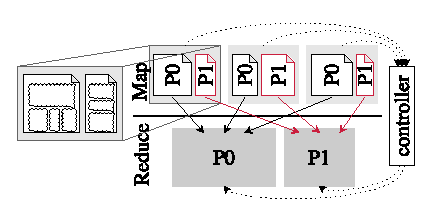
\includegraphics[width=0.5\textwidth]{costModel}
    \caption{Left reducer gets more work than right reducer}\label{img:costModel}
\end{figure}

\end{frame}

\begin{frame}{Load Balancing~\cite{gufler2011handling}}

\begin{cblock}{Fine Partitioning}
    \citem{} Create $p$ partitions with $p > r$ (number of reducers)

    \citem{} High $p$: better load balancing quality, but more expensive monitoring

    \citem{} Partition assignment using greedy approach

    \citem{} Requires that all map tasks have completed

    $\quad \longrightarrow$ What about reducer slow-start?
\end{cblock}

\vfill

\begin{figure}
    \centering
    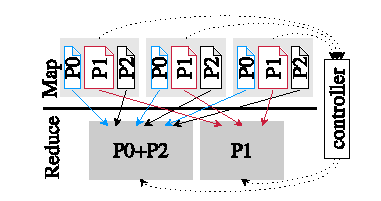
\includegraphics[width=0.5\textwidth]{fineP}
    \caption{P1 most expensive: assigned to dedicated reducer}\label{img:fineP}
\end{figure}

\end{frame}

\begin{frame}{Load Balancing~\cite{gufler2011handling}}

\begin{cblock}{Dynamic Fragmentation}
    \citem{} Split excessively large partitions into $f$ fragments

    \citem{} Fragments can be assigned to different reducers: need data replication

    \citem{} Best partition assignment chosen using cost based strategy:

    \[ \mathcal{C} (R) = \omega (R) \cdot {\left( 1 + \sigma (R) \right)} ^e \]
\end{cblock}

\vfill

\begin{figure}
    \centering
    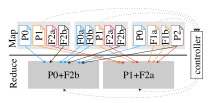
\includegraphics[width=0.5\textwidth]{dynF}
    \caption{P2 replicated on both reducers}\label{img:dynF}
\end{figure}

\end{frame}



%%%%%%%%%%%%%%%%%%%%

\subsection{Handling Reduce Complexity}

\begin{frame}{Outline}
    \tableofcontents[currentsection,currentsubsection]
\end{frame}

\begin{frame}{SkewTune~\cite{Kwon:2012:SMS:2213836.2213840}}
  \begin{cblock}{SkewTune caracteristics}
    \citem{} A solution to the data skew problem from uneven distributions

    \citem{} Does not require rewriting existing map-reduce applications

    \citem{} Does not rely on synchronization barriers
  \end{cblock}
  \vfill
  \begin{cblock}{Principle}
    \citem{} Late skew detection: when a slot is available

    \citem{} Detects one straggler, i.e.\ a task such that $\frac{t}{2} > \omega$

    \citem{} Repartitions the rest of the task on the two slots
  \end{cblock}
\end{frame}

\begin{frame}{SkewTune~\cite{Kwon:2012:SMS:2213836.2213840}}
  \begin{cblock}{Repartionionning}
    \citem{} Use srange partionning

    \citem{} Saves a straggler's output

    \citem{} Repartitions only the unprocessed data
  \end{cblock}
\end{frame}

%%%%%%%%%%%%%%%%%%%%

\subsection{Other Approaches Overview}

\begin{frame}{Outline}
    \tableofcontents[currentsection,currentsubsection]
\end{frame}

\begin{frame}{Overview of other approaches}
\todo{ brief overview of some original / different approaches cited in related work of the papers? }
\end{frame}

%%%%%%%%%%%%%%%%%%%%%%%%%%%%%%%%%%%%%%%%%%%%%%%%%%%%%%%%%%%%

\section{Conclusion}

%%%%%%%%%%%%%%%%%%%%

\begin{frame}{Conclusion}
\todo{}
\end{frame}

%%%%%%%%%%%%%%%%%%%%

\begin{frame}[allowframebreaks]{References}
    \printbibliography%
\end{frame}

%%%%%%%%%%%%%%%%%%%%%%%%%%%%%%%%%%%%%%%%%%%%%%%%%%%%%%%%%%%%

\end{document}
